\newcommand{\depiction}[1]{\parbox{0.7cm}{\includegraphics[height=0.7cm]{../assets/depictions/#1.pdf}}}
\newcommand{\depictionSM}[1]{\parbox{0.6cm}{\includegraphics[height=0.6cm]{../assets/depictions/#1.pdf}}}


\section{Experiments and results}

Now that the engine, the tools and the methodology are defined, we can proceed to the experiments. Experiments will be divided in three sections: motivation, experiment and results. The motivation will explain why I think the experiment is relevant and present possible hypothesis. The experiment will describe configurations to train different models, how they will be evaluated and what are my expectations. The results will present the data, explain whether my hypothesis was correct or not and give a brief conclusion. \\

Every model's training configuration is defined by the following variables:

\begin{itemize}
\item \textbf{Feature set}: Determinates the encoding of the position, and thus the number of inputs of the model. It conditions which patterns the network can learn. Experimenting with this is the main focus of this thesis.

\item \textbf{Network architecture}: The size of each layer in the network. The first layer (L1) is the feature transformer and it is efficiently updated. The following layer (L2) should be tiny due the NNUE architecture. The size of the model (its complexity) roughly determinates how many patterns the network can learn.

\item \textbf{Dataset}: The positions to train on. The dataset used is explained in detail in chapter 5. In summary, there are 48.5 billion positions to train on and the dataset remains constant across all runs. About 5 million positions are used for validation.

% no me gusta la palabra computed...
\item \textbf{Training method}: Can choose to use either score targets or PQR triplets. This determinates the format of the samples as well as the loss function. All experiments will train using score targets, unless specified. Methods were explained in detail in chapter 5.

\item \textbf{Training hyperparameters}: The usual machine learning hyperparameters for training, such as batch size, learning rate and scheduler. I used the same epoch size used in Stockfish, where each epoch is 100 million positions. Each training run will last for 256 epochs, which means the network is trained in 25.6 billion positions (recall that some of the original 48.5 billion dataset are skipped).
\end{itemize}

Once training is completed, the models will be evaluated depending on the experiment. To assess the performance of a model or to compare a set of models, the following indicators are used:

\begin{itemize}
\item \textbf{Loss}: The training and validation loss are used to detect overfitting and other possible problems. It can't be used to measure the performance of a model. Bigger models must have much better predictions to outweight the cost of having slower inferences and thus less node visits. It's a tradeoff.

\item \textbf{Puzzle accuracy}: The percentage of moves correctly predicted by the engine in Lichess puzzles. Each puzzle may contain multiple moves, and the engine has 100ms per move. Since the engine is not that strong, it does not solve 100\% of puzzles like many other engines do, so I expect differences in this metric to be good indicators. A small set of puzzles is used during training as (a very bad) proxy for the engine's strength, to have early insight of the strength and to detect catastrophic failures that did arise. A bigger set of 85000 puzzles is used after training.

\item \textbf{Relative ELO rating}: A tournament is played between different models to determine their relative strength. Ordo is used to compute the ELO of each model based on the results of the tournament. This is the most important metric, as it is the most reliable way to compare the strength of engines.

% \item \textbf{Inference performance (infs/s)}:

\item \textbf{Training duration}: The amount of time it takes to train a model. This is a one time operation and it does not affect the performance of a model. However, it does condition which and how many experiments I can run.
\end{itemize}

All networks that are not in the first experiment (the baseline), are trained 4 times and a tournament is played between the epoch 192 and 256 of each network (8 networks in total). I have observed a difference of 30 elo points between runs, so this step is crucial to have sensible results. In the appendix are the results of each run and tournament.

\subsection{Baseline}

\textbf{Motivation.} Experiments that will follow will focus on trying out different feature sets, so it is natural to keep every other variable constant. Since the dataset is fixed and the feature set is going to be changing, it remains to find acceptable values for the network architecture and the training hyperparameters. 

Due time and resources constraints, I decided to set the training hyperparameters to   (similar) values which give good results in the official Stockfish trainer: \textbf{a batch size of 16384, a learning rate of 0.0005 and a exponential decay factor of 0.99}. This values showed acceptable results during early stages of development and will remain fixed for all runs.

It remains to find a good network architecture. Bigger networks may have lower loss and predict better, but they will also have slower inferences. This is the tradeoff between inference time and node visits (more depth), which are also affected by the quality of the prediction due to better pruning. So the model must be so much better to compensate the slowdown in inference. \\

\textbf{Experiment.}  In this first experiment I will try different sizes of L1 and L2,  to find an acceptable tradeoff for future experiments. I will run a grid search with L1 $\in \{256, 512, 1024, 2048\}$ and L2 $\in \{32, 64, 128, 256\}$. The feature set used to train will be \featureset{All}, the canonical set with 768 features.

I expect that there will be a model that performs best and other models that are smaller (need stronger predictions) and bigger (need speed to visit more nodes) perform worse. \\

\textbf{Results.} Looking at the result heatmaps in Figure \ref{fig:baseline_heatmaps}, the first thing to notice is that training and validation losses behave as expected. If the model is more complex, meaning the number of parameters (which is dominated by $768*L1+L1*L2$) is higher, the loss is lower and the model predicts better.

When the models are loaded into the engine and evaluated in a tournament, we can see that when L2 drops, the performance drops dramatically. This is due the fact that the inference time is mostly dominated by L2. This result suggests that it may be a good idea explore even lower values of L2, such as 16 or even 8. However, the SIMD implementation requires L2 to be a multiple of 32 so it needs a refactor to keep being fast. So, instead of fiddling further with SIMD I decided to \textbf{keep L2 at 32}.

\begin{figure}[H]
\centering
\makebox[\textwidth]{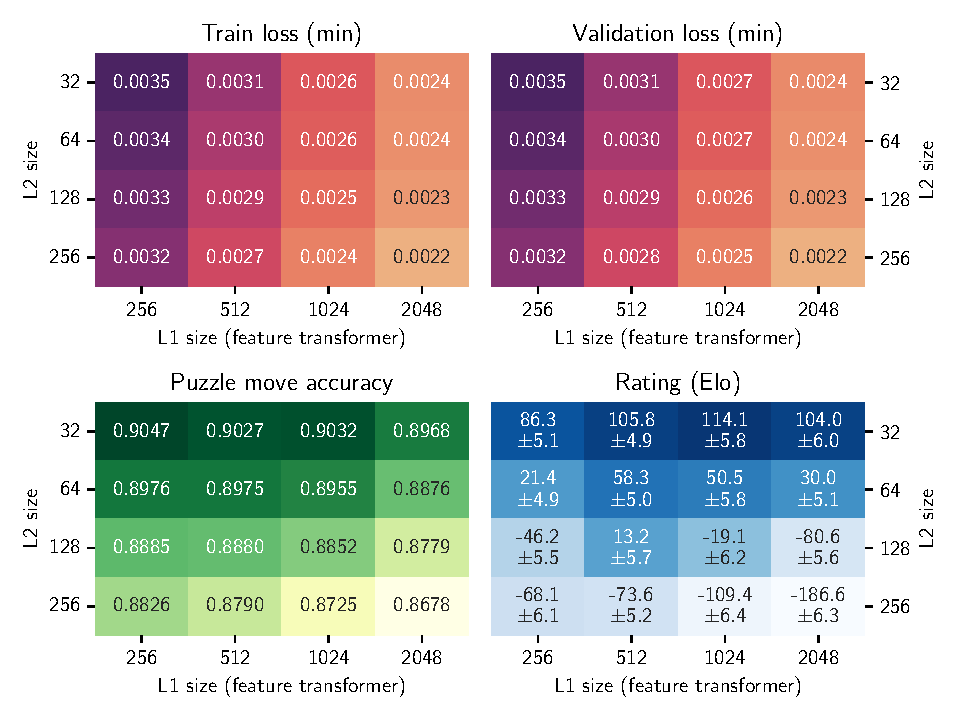
\includegraphics[width=\textwidth]{./dynamic/output/baseline_heatmaps.pdf}}
\captionsetup{justification=centering}
\caption{Network architecture sweep results (L1 $\times$ L2).\\ Table with details in Appendix \ref{appendix:baseline}.}
\label{fig:baseline_heatmaps}
\end{figure}

If L2 is kept constant, the best L1 is not the smallest nor biggest. If L2 $=64$ or L2 $=128$ there is a clear lead of L1 $=512$ in both. In the case of L2 $=32$, the best L1 is not clear because the differences in rating are small and are within margin of error, excluding L1 $=256$ which is definitely wrose. Because training lower values of L1 is faster I opted for \textbf{L1} $\bm{=512}$ due the difference being small and being the best in other L2 values.

So, further experiments will use L1 $=512$ and L2 $=32$. For reference, Stockfish currently uses L1=2560, and employ (lots of) more tricks to make it even faster. The values selected here are specific to the current implementation of the engine, since it may change if more optimizations are made (tradeoff is altered). For this reason, no further modifications to the engine were made after starting with the experiments. We can now proceed with more interesting experiments.

\subsection{Axis encodings}
\label{sec:axis_encoding}

\textbf{Motivation.} Looking back at the networks generated by \featureset{All} in baseline runs, the learned weigths of most neurons in the feature transformer layer (L1) are related with the movement pattern of the pieces. Let's take the example in Figure \ref{fig:rook_weights}, which depicts the \featureset{Square} part of the features where the role is \symrook\ Rook.

\begin{figure}[h]
\centering
\subfloat[\centering $\white$ White]{{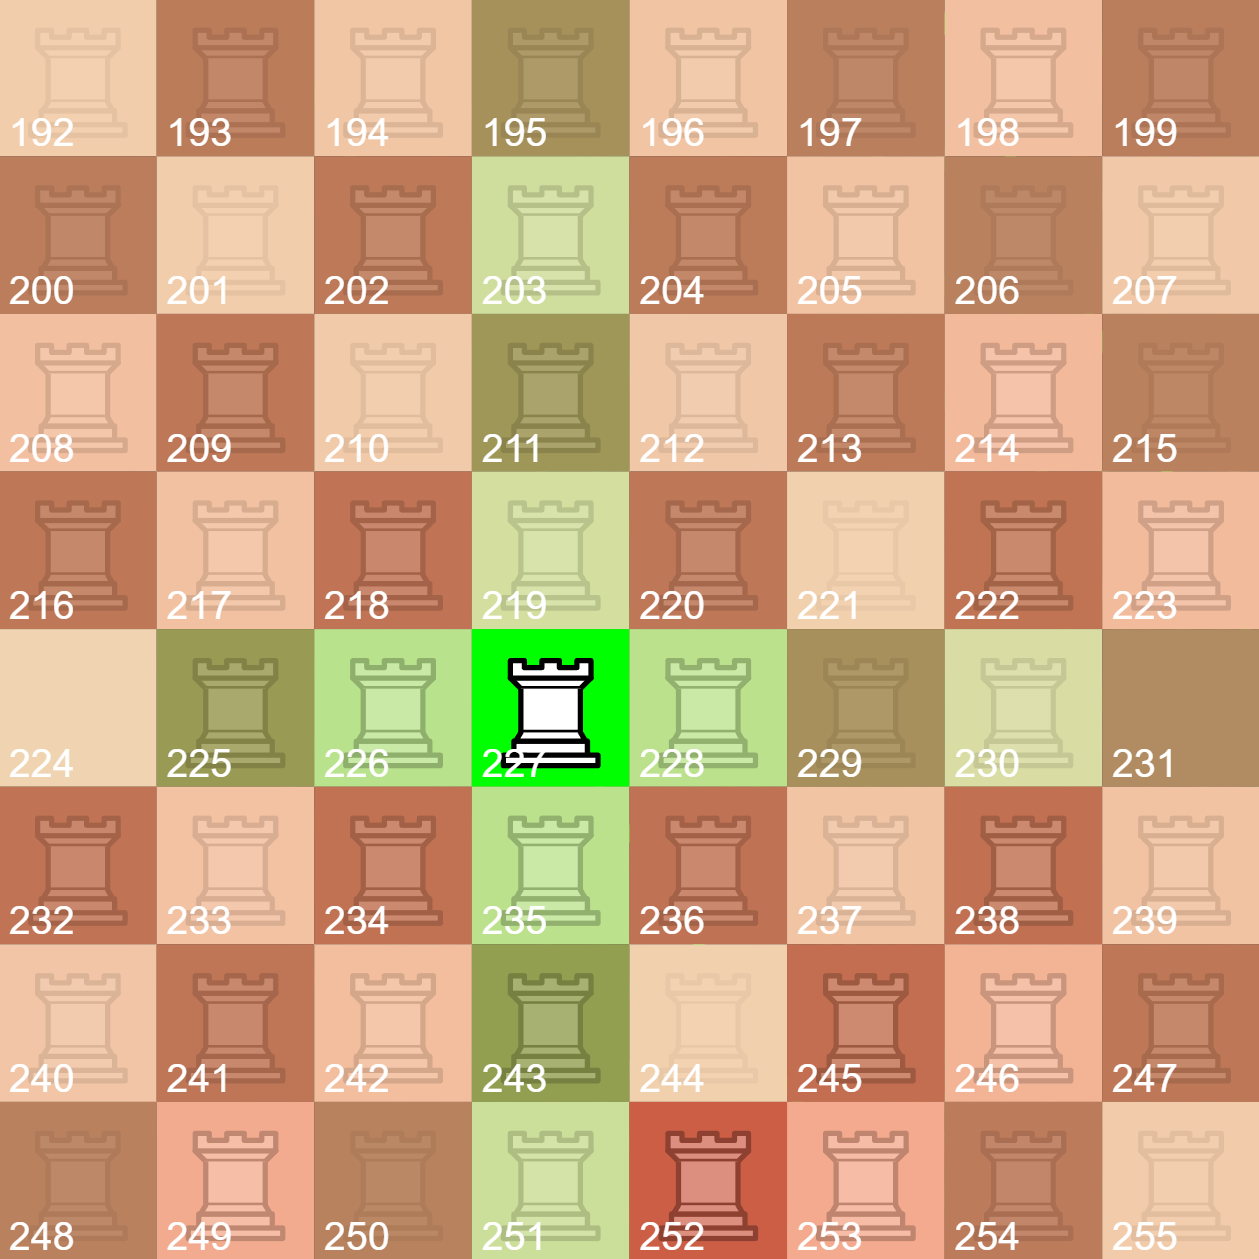
\includegraphics[width=7cm]{../assets/results/piece_weights/white_rook_weights.png} }}%
\qquad
\subfloat[\centering $\black$ Black]{{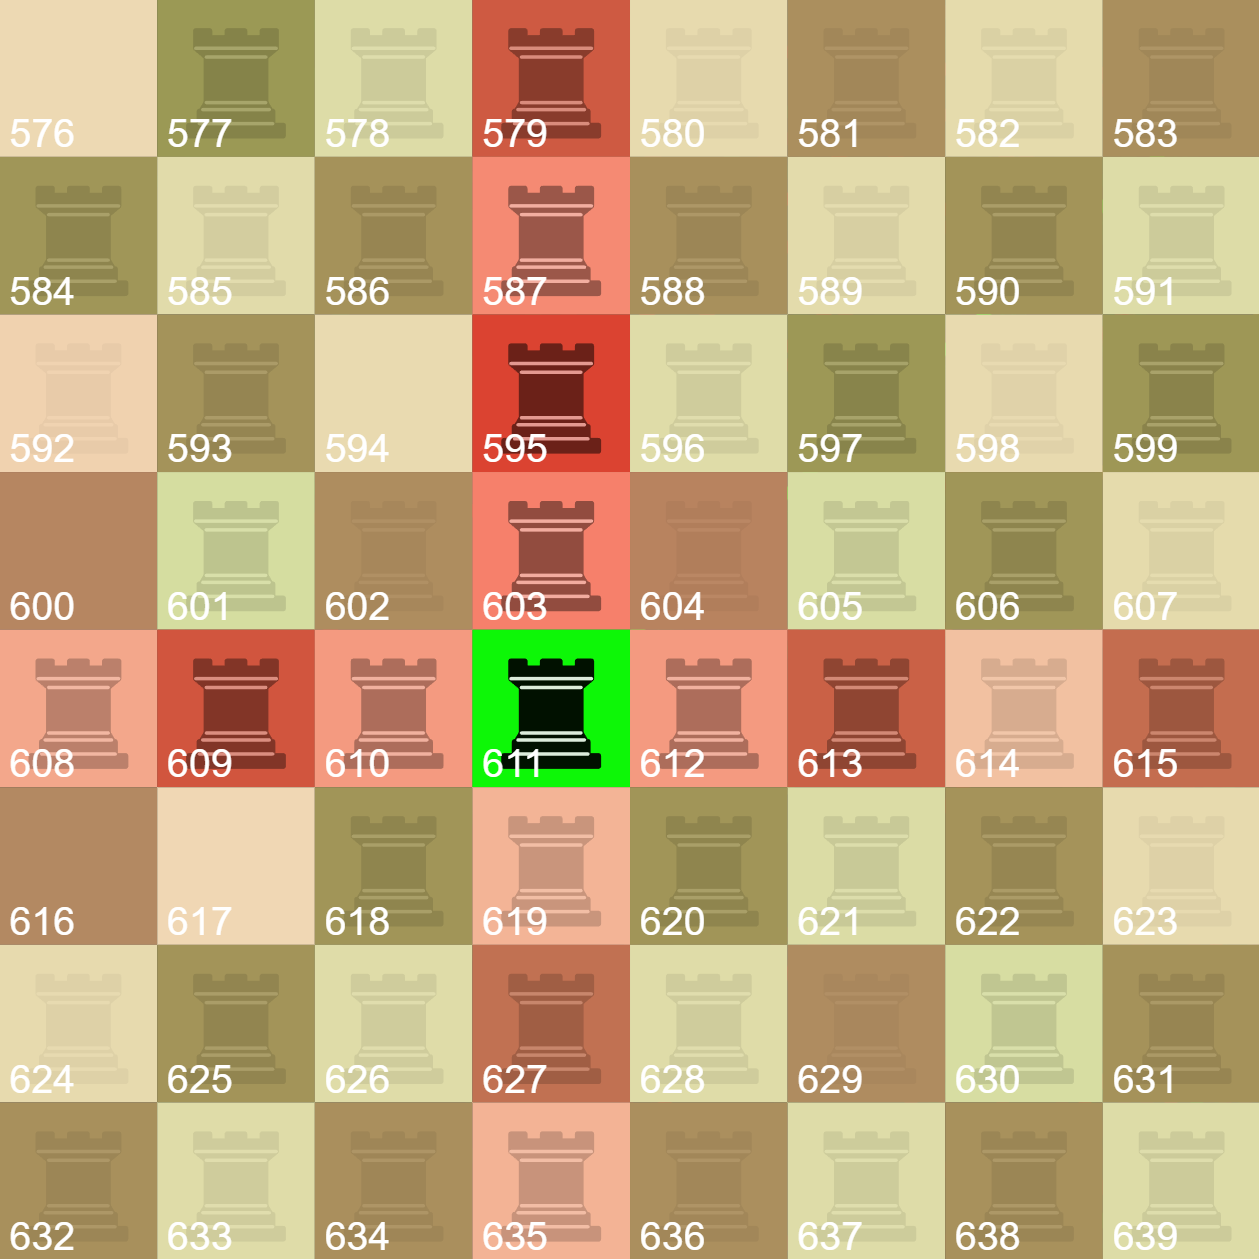
\includegraphics[width=7cm]{../assets/results/piece_weights/black_rook_weights.png} }}%
\caption{Weights of \textbf{a neuron} in the L1 layer, which are connected to features in \featureset{All} where the role is $\rook$ Rook. The intensity represents the weight value, and the color represents the sign (although not relevant).}
\label{fig:rook_weights}
\end{figure}

This particular neuron learned to recognize the presence of a \symrook\ Rook, affected by the pattern of another potential rook in the same file or rank (other pieces may be involved but I am focusing on rooks for the example). Doing so, it had to relate one feature for every potential square where a rook could be for that specific center location, which restrains the network from learning more complex patterns and it is harder to train, because you need more samples to account for all possible combinations.

What if we add a feature which describes \enquote{\textit{there is a $\white$ White $\rook$ Rook in the 4th rank}}? Certainly, this would make the network's job easier, as it would only need to learn the presence of rooks in the corresponding file or rank, instead of every square. This idea can be extrapolated to diagonals, to ease patterns with $\bishop$ Bishops and the $\queen$ Queen.

More examples of this behaviour can be found in Appendix \ref{appendix:axis_samples}, showcasing diagonal patterns and the $\knight$ Knight movements, although they do not move straight through axes. \\

\textbf{Experiment.} I built blocks of features for each natural axis of a chess board, which coincide with the movement pattern of the pieces:

\begin{table}[H]
\centering
\begin{tabular}{cccc}
\depiction{H} & \depiction{V} & \depiction{D1} & \depiction{D2} \\
Horizontal & Vertical & Diagonal 1 & Diagonal 2 \\
(across files) & (across ranks) &  & 
\end{tabular}
\end{table}

% The canonical \featureset{All} feature set encodes each piece's position using the square it is located. Note that this is the same thing as encoding the position for a piece $P$ as $\featureset{File}_{P} \times \featureset{Rank}_{P}$. So the position of each piece is determined using the vertical (across ranks) and horizonal (across files) axes.

In table \ref{tab:axes_blocks} I present the feature blocks. Each block will encode whether there is a piece with the role and color in a specific location along that axis, as explained in the example.

\begin{table}[H]
\caption{Axes feature blocks}
\label{tab:axes_blocks}
\centering

\newcommand{\fullrolecolor}{$\times$ $\featureset{Role}_{P} \times \featureset{Color}_{P}$}

\begin{tabular}{cccccc}
\toprule
\bf Depiction & \bf Block name & \multicolumn{2}{c}{\makecell{\bf Definition\\for every piece $P$ in the board}} & \bf \makecell{Number of\\features} \\
\toprule
\depiction{H} & $\featureset{H}$ & $\featureset{File}_{P}$ & \fullrolecolor & 96 \\
\depiction{V} & $\featureset{V}$ & $\featureset{Rank}_{P}$ & \fullrolecolor & 96 \\
\depiction{D1} & $\featureset{D1}$ & $\featureset{Diag1}_{P}$ & \fullrolecolor & 180 \\
\depiction{D2} & $\featureset{D2}$ & $\featureset{Diag2}_{P}$ & \fullrolecolor & 180 \\
\bottomrule
\end{tabular}

\end{table}


With this blocks, I built different feature sets (listed in table \ref{tab:axis_encoding}): one group of feature sets is just combinations of all the blocks, and another group which is the same as the first but alongside the \featureset{All} feature set (here treated as a block). The second group is the aim of the experiment, it has the classic \featureset{All} feature set but includes the axis blocks to see if the network can benefit from them. The first group, which does not include \featureset{All} is to know how far the network can go only with this blocks alone.

\begin{table}[H]
\caption{Axis encodings feature sets}
\label{tab:axis_encoding}
\centering

\newcommand{\rolecolor}{$\times$ $\featureset{R}_{P} \times \featureset{C}_{P}$}

\begin{tabular}{ccc}
\toprule
\bf Depiction & \bf Feature set & \bf \makecell{Number of\\features} \\
\toprule
\depiction{H} $\oplus$ \depiction{V} & $\featureset{H} \oplus \featureset{V}$ & 192 \\
\midrule
\depiction{D1} $\oplus$ \depiction{D2} & $\featureset{D1} \oplus \featureset{D2}$ & 360 \\
\midrule
\depiction{H} $\oplus$ \depiction{V} $\oplus$ \depiction{D1} $\oplus$ \depiction{D2} & $\featureset{H} \oplus \featureset{V}$ $\oplus$ $\featureset{D1} \oplus \featureset{D2}$ & 552 \\
\midrule
% ------------------------------------
\midrule
\featureset{All} $\oplus$ \depiction{H} $\oplus$ \depiction{V} & $\featureset{All} \oplus \featureset{H} \oplus \featureset{V}$ & 960 \\
\midrule
\featureset{All} $\oplus$ \depiction{D1} $\oplus$ \depiction{D2} & $\featureset{All} \oplus \featureset{D1} \oplus \featureset{D2}$ & 1128 \\
\midrule
\featureset{All} $\oplus$ \depiction{H} $\oplus$ \depiction{V} $\oplus$ \depiction{D1} $\oplus$ \depiction{D2} & \featureset{All} $\oplus$ \featureset{H} $\oplus$ \featureset{V} $\oplus$ \featureset{D1} $\oplus$ \featureset{D2} & 1320 \\
\bottomrule

\end{tabular}
\end{table}

I expect that the feature sets that are sums of single axes ($\depictionSM{H} \oplus \depictionSM{V}, \depictionSM{D1} \oplus \depictionSM{D2}$ and $\depictionSM{H} \oplus \depictionSM{V} \oplus \depictionSM{D1} \oplus \depictionSM{D2}$) will perform worse overall, since to capture the exact position of pieces in the board, the network will have to learn to relate at least two features for every location. This information is already available when \featureset{All} is present.

The feature sets that include \featureset{All} (\featureset{All} $\oplus \hdots$) should perform better than without, providing that the idea explained in the motivation holds.

For each of the proposed feature sets, I will train a network and evaluate its performance relative to each other using a tournament. I expect to see them ranked in the reverse order as presented in the table (more extra axes better). \\

\textbf{Results.} The results in table \ref{tab:axis_results} show that indeed, adding the axes blocks make the network validation loss slightly lower, from 0.00316 in \featureset{All} to 0.00307 including all four blocks. However, this improvement in loss is not significant enough to make the network stronger to compensate the (small) performance hit of having more features. As you can see in the table, including more axes makes the loss decrease slightly yet the rating decreases by a huge factor.

All three feature sets that do not include \featureset{All} unsuprisingly perform much, much worse even having less features. The feature set \featureset{H+V+D1+D2} has a 25\% higher loss than \featureset{All} and $172.5 \pm 4.8$ less rating than \featureset{All}. The other feature sets in this group perform even worse, as it was expected.

I discovered that the accuracy of puzzles is not a good a proxy of an engine's strength, given that there is a 474 rating difference yet 3\% a difference in move accuracy. I believe that the reason lies on the fact that puzzles may be more strategic than positional. I will drop the puzzle accuracy metric in future experiments.

\begin{table}[H]
\caption{Axis encodings results}
\label{tab:axis_results}
\centering

% 1 256-eval_16384_(hv[768]→512)x2→32→1.nn          :     0.0   ----  22665.5   32456    70      96
% 2 256-eval_16384_(hv+h+v[960]→512)x2→32→1.nn      :    -4.6    5.0  22474.0   32456    69     100
% 3 256-eval_16384_(hv+d1+d2[1128]→512)x2→32→1.nn   :   -33.3    5.0  21260.5   32456    66     100
% 4 256-eval_16384_(hv+h+v+d1+d2[1320]→512)x2→32→1.nn   :   -57.7    4.8  20207.5   32458    62     100
% 5 256-eval_16384_(h+v+d1+d2[552]→512)x2→32→1.nn   :  -172.5    4.8  15176.0   32456    47     100
% 6 256-eval_16384_(h+v[192]→512)x2→32→1.nn         :  -368.1    5.7   7527.0   32460    23     100
% 7 256-eval_16384_(d1+d2[360]→512)x2→32→1.nn       :  -474.5    6.4   4289.5   32458    13     ---

% Network: 256-eval_16384_(d1+d2[360]→512)x2→32→1.nn Accuracy: 0.851789055191768
% Network: 256-eval_16384_(h+v+d1+d2[552]→512)x2→32→1.nn Accuracy: 0.8748684518241348
% Network: 256-eval_16384_(h+v[192]→512)x2→32→1.nn Accuracy: 0.8618817235734331
% Network: 256-eval_16384_(hv+d1+d2[1128]→512)x2→32→1.nn Accuracy: 0.8814458606173995
% Network: 256-eval_16384_(hv+h+v+d1+d2[1320]→512)x2→32→1.nn Accuracy: 0.8766955098222639
% Network: 256-eval_16384_(hv[768]→512)x2→32→1.nn Accuracy: 0.8865762394761459
% Network: 256-eval_16384_(hv+h+v[960]→512)x2→32→1.nn Accuracy: 0.8851511342376053

\begin{tabular}{cccccc}
\toprule
\bf Feature set  & \bf \makecell{Number\\of features} & \makecell{\bf Val. loss\\\textit{min}} & \makecell{\bf Rating\\\textit{elo (rel. to \featureset{All})}} & \makecell{\bf Puzzles\\\textit{move acc.}} \\
\toprule
\depiction{H} $\oplus$ \depiction{V} & 192 & 0.00581 & -368.1 $\pm$ 5.7 & 0.8618 \\
\midrule
\depiction{D1} $\oplus$ \depiction{D2} & 360 & 0.00670 & -474.5 $\pm$ 6.4 & 0.8517 \\
\midrule
\makecell{\depiction{H} $\oplus$ \depiction{V} $\oplus$ \\ \depiction{D1} $\oplus$ \depiction{D2}} & 552 & 0.00389 & -172.5 $\pm$ 4.8 & 0.8748 \\
\midrule
% ------------------------------------
\midrule
\featureset{All} (reference) & 768 & 0.00316 & \textbf{0.0} & 0.8865 \\
\midrule
\featureset{All} $\oplus$ \depiction{H} $\oplus$ \depiction{V} & 960 & 0.00308 & -4.6 $\pm$ 5.0 & 0.8851 \\
\midrule
\featureset{All} $\oplus$ \depiction{D1} $\oplus$ \depiction{D2} & 1128 & 0.00309 & -33.3 $\pm$ 5.0 & 0.8814 \\
\midrule
\makecell{\featureset{All} $\oplus$ \depiction{H} $\oplus$ \depiction{V} \\ \hspace{0.75cm} $\oplus$ \depiction{D1} $\oplus$ \depiction{D2}} & 1320 & \textbf{0.00307} & -57.7 $\pm$ 4.8 & 0.8766 \\
\bottomrule

\end{tabular}
\end{table}

The next experiment will focus on adding more specific features, instead of more broad ones.


\subsection{Pairwise axes}

\textbf{Motivation.} Imagine that in a file there are three pieces: an enemy $\symrook$ Rook, a $\sympawn$ Pawn and a $\symknight$ Knight. There are many possible configurations for these pieces on the file. The influence in the evaluation by those pieces is very related with the position of pieces everywhere else, however I want to see if to understand a single file, the actual position of the pieces is less important than the relative order between them: $\sympawn\symknight\symrook, \sympawn\symrook\symknight, \symknight\sympawn\symrook, \symknight\symrook\sympawn, \symrook\sympawn\symknight, \symrook\symknight\sympawn$. In other words, provide the network features based on the order of the pieces instead of the actual position. This way, I believe that the network can pick up whether pieces are pinned, protected by other pieces or can attack other pieces.

I propose to make a feature for each possible pair of adjacent role and color over an axis. Lets consider the \textit{a} file (vertical axis), following the example before:

\storechessboardstyle{smallvert}{
    tinyboard,
    maxfield=a8,
    showmover=false,
    hmargin=false,
    hlabel=false,
    boardfontsize=15pt,
}

\newcommand{\raiseby}{-11.5ex}

\begin{figure}[H]
\centering

\begin{tabular}{ccc}

\raisebox{\raiseby}{\chessboard[
    style=smallvert,
    addblack={Ra7},
    addwhite={na3,pa4},
]}
\raisebox{\raiseby}{\chessboard[
    style=smallvert,
    addblack={Ra8},
    addwhite={na2,pa3},
]}
\raisebox{\raiseby}{\chessboard[
    style=smallvert,
    addblack={Ra6},
    addwhite={na3,pa4},
]}
\raisebox{\raiseby}{\chessboard[
    style=smallvert,
    addblack={Ra5},
    addwhite={na1,pa3},
]}
\raisebox{\raiseby}{\chessboard[
    style=smallvert,
    addblack={Ra6},
    addwhite={na2,pa3},
]}

$\hdots$

&
$ \rightarrow$
&

\raisebox{-9.5ex}{\chessboard[
    blackfieldcolor=white,
    blackfieldmaskcolor=white,
    maxfield=a8,
    style=smallvert,
    vlabel=false,
    border=false,
    trim=false,
    opacity=0.6,
    addblack={Ra6},
    addwhite={na2,pa4},
    %
    color=red,
    shortenend=1.88ex,shortenstart=1.88ex, % espacio
    padding=-1ex,
    markstyle=leftborder,
    linewidth=0.4ex,
    markregion=a4-a6,
    linewidth=1.6ex,
    pgfstyle=circle,
    markfields={a4,a6},
    %
    color=blue,
    shortenend=1.88ex,shortenstart=1.88ex, % espacio
    padding=-1ex,
    markstyle=leftborder,
    linewidth=0.4ex,
    markregion=a2-a4,
    linewidth=1.6ex,
    pgfstyle=circle,
    markfields={a2,a4},
    %
]}

\\

\makecell{Different configurations,\\similar situation} &  & \makecell{The same two features\\(blue pair and red pair)}

\end{tabular}
\end{figure}

There are many configurations for the three pieces and the idea is to collapse all of these into two features: the pair of pieces ($\symrook$$\black$, $\sympawn$$\white$) and the pair of pieces ($\sympawn$$\white$, $\symknight$$\white$). This way, the network can learn that the $\symrook$ Rook can capture the $\sympawn$ Pawn, and that the $\symknight$ Knight is protected behind the $\sympawn$ Pawn. The network can learn this situation using two features instead of learning it for every possible configuration.

In contrast to the previous experiment where the features were more general (\textit{\enquote{there is a $\white$ White $\rook$ Rook in the 4th rank}}) the proposed features here are more specific: \textit{\enquote{there is a $\black$ Black $\rook$ Rook next to a $\white$ White $\sympawn$ Pawn in the \enquote{a} file}}. \\

\textbf{Experiment.} I developed two feature blocks: for the horizonal and vertical axis. The blocks are defined in table \ref{tab:pairwise_blocks}:

\begin{table}[H]
\caption{Pairwise feature blocks}
\label{tab:pairwise_blocks}
\centering

\begin{tabular}{ccccc}
\toprule
\bf Depiction & \bf \makecell{Block\\name} & \bf Definition & \bf \makecell{Num. of\\features} \\
\toprule
\depiction{PH} & PH & \makecell{
\vspace{0.2cm}
$(\featureset{Ranks} \times (\featureset{Roles} \times \featureset{Colors}) \times (\featureset{Roles} \times \featureset{Colors}))_{P}$ \\
P($\langle r, r_1, c_1, r_2, c_2 \rangle$): there is a piece in rank $r$ with role $r_1$\\ and color $c_1$ to the left of a piece with role $r_2$ and color $c_2$
} & 1152 \\
\toprule
\depiction{PV} & PV & \makecell{
\vspace{0.2cm}
$(\featureset{Files} \times (\featureset{Roles} \times \featureset{Colors}) \times (\featureset{Roles} \times \featureset{Colors}))_Q$ \\
Q($\langle f, r_1, c_1, r_2, c_2 \rangle$): there is a piece in file $f$ with role $r_1$\\ and color $c_1$ below a piece with role $r_2$ and color $c_2$
} & 1152 \\
\bottomrule
\end{tabular}
\end{table}

Note that it is important to consider the order of the pieces in the pair, as expressed in the direction of the definition (left and below).
This makes sure features are not mirrored, since we want to differentiate between both. In code this is handled by iterating over the pieces and building the pair in the same order every time.

The following figure shows what pairs of pieces (features) are considered for the horizonal and vertical axes in a complete board:

\begin{figure}[H]
\centering
\begin{tabular}{cc}

\raisebox{-7ex}{\chessboard[
    setfen=2r4k/p5p1/Kpqp3p/8/1PP2Q2/P2P1RP1/8/8 b - - 12 45,
    showmover=false,
    opacity=0.6,
    %
    % TEMPLATE HORIZONTAL
    %color=red,
    %shortenend=1.88ex,shortenstart=1.88ex, % espacio
    %padding=-1ex,
    %markstyle=topborder,
    %linewidth=0.4ex,
    %markregion=d6-d3,
    %linewidth=1.6ex,
    %pgfstyle=circle,
    %markfields={d6,d3},
    %
    color=red,
    shortenend=1.88ex,shortenstart=1.88ex, % espacio
    padding=-1ex,
    markstyle=topborder,
    linewidth=0.4ex,
    markregion=a3-d3,
    linewidth=1.6ex,
    pgfstyle=circle,
    markfields={a3,d3},
    %
    color=red,
    shortenend=1.88ex,shortenstart=1.88ex, % espacio
    padding=-1ex,
    markstyle=topborder,
    linewidth=0.4ex,
    markregion=f3-g3,
    linewidth=1.6ex,
    pgfstyle=circle,
    markfields={f3,g3},
    %
    color=blue,
    shortenend=1.88ex,shortenstart=1.88ex, % espacio
    padding=-1ex,
    markstyle=topborder,
    linewidth=0.4ex,
    markregion=d3-f3,
    linewidth=1.6ex,
    pgfstyle=circle,
    markfields={d3,f3},
    %
    color=red,
    shortenend=1.88ex,shortenstart=1.88ex, % espacio
    padding=-1ex,
    markstyle=topborder,
    linewidth=0.4ex,
    markregion=b4-c4,
    linewidth=1.6ex,
    pgfstyle=circle,
    markfields={b4,c4},
    %
    color=blue,
    shortenend=1.88ex,shortenstart=1.88ex, % espacio
    padding=-1ex,
    markstyle=topborder,
    linewidth=0.4ex,
    markregion=c4-f4,
    linewidth=1.6ex,
    pgfstyle=circle,
    markfields={c4,f4},
    %
    color=red,
    shortenend=1.88ex,shortenstart=1.88ex, % espacio
    padding=-1ex,
    markstyle=topborder,
    linewidth=0.4ex,
    markregion=a6-b6,
    linewidth=1.6ex,
    pgfstyle=circle,
    markfields={a6,b6},
    %
    color=red,
    shortenend=1.88ex,shortenstart=1.88ex, % espacio
    padding=-1ex,
    markstyle=topborder,
    linewidth=0.4ex,
    markregion=c6-d6,
    linewidth=1.6ex,
    pgfstyle=circle,
    markfields={c6,d6},
    %
    color=blue,
    shortenend=1.88ex,shortenstart=1.88ex, % espacio
    padding=-1ex,
    markstyle=topborder,
    linewidth=0.4ex,
    markregion=b6-c6,
    linewidth=1.6ex,
    pgfstyle=circle,
    markfields={b6,c6},
    %
    color=blue,
    shortenend=1.88ex,shortenstart=1.88ex, % espacio
    padding=-1ex,
    markstyle=topborder,
    linewidth=0.4ex,
    markregion=d6-h6,
    linewidth=1.6ex,
    pgfstyle=circle,
    markfields={d6,h6},
    %
    color=red,
    shortenend=1.88ex,shortenstart=1.88ex, % espacio
    padding=-1ex,
    markstyle=topborder,
    linewidth=0.4ex,
    markregion=a7-g7,
    linewidth=1.6ex,
    pgfstyle=circle,
    markfields={a7,g7},
    %
    color=blue,
    shortenend=1.88ex,shortenstart=1.88ex, % espacio
    padding=-1ex,
    markstyle=topborder,
    linewidth=0.4ex,
    markregion=c8-h8,
    linewidth=1.6ex,
    pgfstyle=circle,
    markfields={c8,h8},
]}

&

\raisebox{-7ex}{\chessboard[
    setfen=2r4k/p5p1/Kpqp3p/8/1PP2Q2/P2P1RP1/8/8 b - - 12 45,
    showmover=false,
    opacity=0.6,
    %
    % TEMPLATE VERTICAL
    %color=red,
    %shortenend=1.88ex,shortenstart=1.88ex, % espacio
    %padding=-1ex,
    %markstyle=leftborder,
    %linewidth=0.4ex,
    %markregion=d6-d3,
    %linewidth=1.6ex,
    %pgfstyle=circle,
    %markfields={d6,d3},
    %
    color=red,
    shortenend=1.88ex,shortenstart=1.88ex, % espacio
    padding=-1ex,
    markstyle=leftborder,
    linewidth=0.4ex,
    markregion=a3-a6,
    linewidth=1.6ex,
    pgfstyle=circle,
    markfields={a3,a6},
    %
    color=blue,
    shortenend=1.88ex,shortenstart=1.88ex, % espacio
    padding=-1ex,
    markstyle=leftborder,
    linewidth=0.4ex,
    markregion=a6-a7,
    linewidth=1.6ex,
    pgfstyle=circle,
    markfields={a6,a7},
    %
    color=red,
    shortenend=1.88ex,shortenstart=1.88ex, % espacio
    padding=-1ex,
    markstyle=leftborder,
    linewidth=0.4ex,
    markregion=b4-b6,
    linewidth=1.6ex,
    pgfstyle=circle,
    markfields={b4,b6},
    %
    color=red,
    shortenend=1.88ex,shortenstart=1.88ex, % espacio
    padding=-1ex,
    markstyle=leftborder,
    linewidth=0.4ex,
    markregion=c4-c6,
    linewidth=1.6ex,
    pgfstyle=circle,
    markfields={c4,c6},
    %
    color=blue,
    shortenend=1.88ex,shortenstart=1.88ex, % espacio
    padding=-1ex,
    markstyle=leftborder,
    linewidth=0.4ex,
    markregion=c6-c8,
    linewidth=1.6ex,
    pgfstyle=circle,
    markfields={c6,c8},
    %
    color=red,
    shortenend=1.88ex,shortenstart=1.88ex, % espacio
    padding=-1ex,
    markstyle=leftborder,
    linewidth=0.4ex,
    markregion=d3-d6,
    linewidth=1.6ex,
    pgfstyle=circle,
    markfields={d3,d6},
    %
    color=red,
    shortenend=1.88ex,shortenstart=1.88ex, % espacio
    padding=-1ex,
    markstyle=leftborder,
    linewidth=0.4ex,
    markregion=f3-f4,
    linewidth=1.6ex,
    pgfstyle=circle,
    markfields={f3,f4},
    %
    color=red,
    shortenend=1.88ex,shortenstart=1.88ex, % espacio
    padding=-1ex,
    markstyle=leftborder,
    linewidth=0.4ex,
    markregion=g3-g7,
    linewidth=1.6ex,
    pgfstyle=circle,
    markfields={g3,g7},
    %
    color=red,
    shortenend=1.88ex,shortenstart=1.88ex, % espacio
    padding=-1ex,
    markstyle=leftborder,
    linewidth=0.4ex,
    markregion=h6-h8,
    linewidth=1.6ex,
    pgfstyle=circle,
    markfields={h6,h8},
]}


\\

\makecell{\depiction{PH} Pairwise horizontal (\featureset{PH})} &
\makecell{\depiction{PV} Pairwise vertical (\featureset{PV})}

\end{tabular}
\end{figure}

Since the blocks need at least two pieces to generate a feature, if there is only one piece over an axis, there are no active features. So, this blocks can't be used alone, they need to be combined with other features that provide that information. The most obvious choice is to combine them with the \featureset{All} block.

The feature sets to be evaluated are \featureset{All} $\oplus$ \featureset{PH} (1920 features), \featureset{All} $\oplus$ \featureset{PV} (1920 features) and \featureset{All} $\oplus$ \featureset{PH} $\oplus$ \featureset{PV} (3072 features). Like before, a network will be trained for each feature set and a tournament will be played to determinate the relative elo to the \featureset{All} baseline.

I expect that the networks are able to take advantage of the specific features, enough to conteract the loss in performance due to the big increase in the number of features and slower updates. \\

\textbf{Results.} The results in table \ref{tab:pairwise_results} show that there is a clear difference in performance between \depictionSM{PH} and \depictionSM{PV}. The feature set \featureset{All} $\oplus$ \depictionSM{PV} has a lower loss and rating than its counterpart \featureset{All} $\oplus$ \depictionSM{PH}. It is not clear why the vertical pairs achieve a better rating than the horizontal pairs, since they have a similar amount of feature updates (Appendix \ref{appendix:fs}).

Both \featureset{All} $\oplus$ \depictionSM{PV} and \featureset{All} $\oplus$ \depictionSM{PH} perform worse than \featureset{All}. It seems that the networks were able to take advantage of the pairs, since the loss is lower than the reference. However, it is not enough to conteract the increase in feature updates.

Suprisingly the feature set with both axes (\featureset{All} $\oplus$ \depictionSM{PH} $\oplus$ \depictionSM{PV}) has a similar rating to \featureset{All} $\oplus$ \depictionSM{PV}, probably counteracted by having an even lower loss.

\begin{table}[H]
\caption{Pairwise encodings results}
\label{tab:pairwise_results}
\centering

\begin{tabular}{ccccc}
\toprule
\bf Feature set  & \bf \makecell{Number\\of features} & \makecell{\bf Val. loss\\\textit{min}} & \makecell{\bf Rating\\\textit{elo (rel. to \featureset{All})}} \\
\toprule
\featureset{All} (reference) & 768 & 0.003134 & \textbf{0.0} \\
\midrule
\featureset{All} $\oplus$ \depiction{PH} & 1920 & 0.003033 & -38.2 $\pm$ 4.8 \\
\midrule
\featureset{All} $\oplus$ \depiction{PV} & 1920 & 0.002946 & -8.4 $\pm$ 5.0 \\
\midrule
\featureset{All} $\oplus$ \depiction{PH} $\oplus$ \depiction{PV} & 3072 & \textbf{0.002868} & -37.6 $\pm$ 4.9 \\
\bottomrule
\end{tabular}
\end{table}

Future work could gather some statistics about the pairs and determinate if skipping some pairs is worth it. For example, pairs related to pawns cause many updates since it is the most common piece and may not be that useful. Reducing the amount of pairs would lower the amount of updates and may overtake \featureset{All}.

I did not bother implementing diagonal pairs (\depiction{PD1} and \depiction{PD2}) due the adverse result of the other axes.


\noindent\rule{\textwidth}{1pt}

\vspace{0.2cm}
Up to this point, I have been trying to encode the position of the pieces in different or smarter ways, with no avail. It may seem that the network is able to extract all the information it needs from the most basic \featureset{All} feature set. Making the information available in another form makes no difference, as opposed to what I originally thought.

Further experiments will focus on features not related to the position of the pieces, but to other aspects of the game, inspired by hand crafted evaluations.

\noindent\rule{\textwidth}{1pt}


\subsection{Mobility}

\textbf{Motivation.} Mobility in chess is a measure of the available moves a player can make in a given position. The idea is that if a player has more available moves, the position is stronger. In \cite{slater:1950} it was shown that there is a strong correlation between a player's mobility and the number of games won. This metric has been used extensively in hand crafted evaluations, and I propose to include this information as features for the neural network. \\

\textbf{Experiment.} There are two ways to go about encoding mobility:

\begin{itemize}
\item \textbf{Bitsets (per piece type):} Provide the exact squares each piece type can move to. The number of features would be $64 * 6 * 2 = 768$. The problem with this approach is not the amount of features, but the number of updates to the accumulator per move is very high, which slows down the search.

\begin{figure}[H]
\centering

\begin{tabular}{ccccc}

\raisebox{-7ex}{\chessboard[
    setfen=r5k1/1b1p1ppp/p7/1p1Q4/2p1r3/PP4Pq/BBP2b1P/R4R1K w - - 0 20,
    tinyboard,
    showmover=false,
]}
&

\raisebox{-7ex}{\chessboard[
    tinyboard,
    showmover=false,
    setwhite={ba2,bb2},
    pgfstyle=color,
    opacity=0.8,
    color=blue,
    markfield={b1,c1,c3,d4,e5,f6,g7}
]}

&

\raisebox{-7ex}{\chessboard[
    tinyboard,
    showmover=false,
    addblack={Bb7,Bf2},
    pgfstyle=color,
    opacity=0.8,
    color=blue,
    markfield={c8,c6,d5,a7,b6,c5,d4,e3,e1,g1,g3}
]}

&

\raisebox{-7ex}{\chessboard[
    tinyboard,
    showmover=false,
    setwhite={qd5},
    pgfstyle=color,
    opacity=0.8,
    color=blue,
    markfield={d6,d7,e6,f7,e5,f5,g5,h5,e4,d4,d3,d2,d1,c4,c5,b5,c6,b7}
]}

& $\hdots$

\\

Board &
\makecell{\white White\\\symbishop\ Bishop} &
\makecell{\black Black\\\symbishop\ Bishop} &
\makecell{\white White\\\symqueen\ Queen}

\end{tabular}
\end{figure}


\item \textbf{Counts (per piece type):} Use the number of available moves per piece type as features. This means having a feature for each possible count value, which are a lot less feature updates. To find which values to include as features I computed the total mobility for each piece role in 2 billion boards, shown in figure \ref{fig:mobility}. From the data we can extract the range of values to use as features:

\begin{table}[H]
\centering
\begin{tabular}{c|c|c}
\toprule
\textbf{Piece role} & \textbf{Min} & \textbf{Max} \\
\midrule
\sympawn\ Pawn & 0 & 8+ \\
\symknight\ Knight & 0 & 15+ \\
\symbishop\ Bishop & 0 & 16+ \\
\symrook\ Rook & 0 & 25+ \\
\symqueen\ Queen & 0 & 25+ \\
\symking\ King & 0 & 8 \\
\bottomrule
\end{tabular}
\end{table}

\begin{figure}[H]
\centering
\makebox[\textwidth]{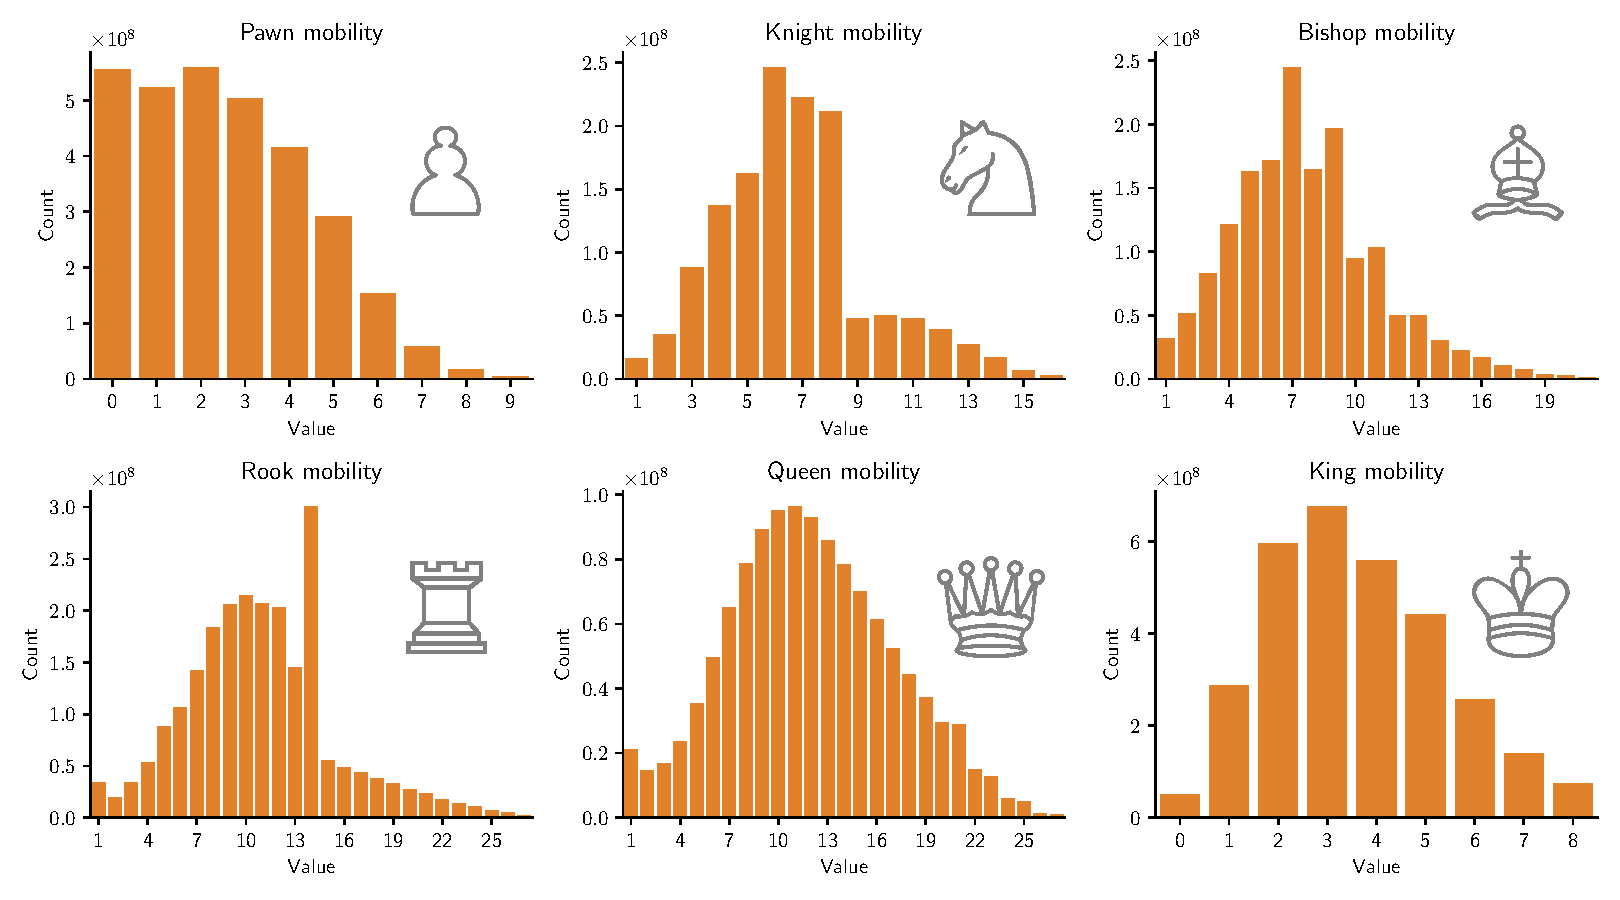
\includegraphics[width=\textwidth]{./dynamic/output/mobility.pdf}}
\caption{Total mobility values for each piece on the board. Computed using 2 billion boards. The value 0 for the \symknight\ Knight, \symbishop\ Bishop, \symrook\ Rook and \symqueen\ Queen has been excluded from the plot, as it is very common.}
\label{fig:mobility}
\end{figure}
\end{itemize}

Each approach was implemented as a block:

\begin{table}[H]
\caption{Mobility feature blocks}
\label{tab:mobility_blocks}
\centering

\begin{tabular}{ccc}
\toprule
\bf Block name & \bf Definition & \bf Number of features \\
\toprule
MB & \makecell{
\vspace{0.2cm}
($\featureset{Squares} \times \featureset{Roles} \times \featureset{Colors})_P$ \\
P($\langle s, r, c \rangle$): there is a piece of role $r$\\ and color $c$ that \textbf{can move to} square $s$
} & 768 \\
\toprule
MC & \makecell{
\vspace{0.2cm}
$(\{0, 1, \hdots\} \times \featureset{Roles} \times \featureset{Colors})_{P}$\\
P($\langle m, r, c \rangle$): the value of mobility for\\
a piece of role $r$ and color $c$ is $m$
} & 206 \\
\bottomrule
\end{tabular}
\end{table}

The blocks will be combined with the \featureset{All} feature set. Neither of the blocks can be used alone, since they do not carry the information to deduce every piece on the board (trivially).

The feature sets to be trained and evaluated are \featureset{All} $\oplus$ \featureset{MB} (1536 features) and \featureset{All} $\oplus$ \featureset{MC} (974 features). Like prior experiments, a network will be trained for each feature set and evaluated in a tournament. \\

\textbf{Results.} The results in table \ref{tab:mobility_results} show that the blocks did not provide features of enough quality to improve the network predictions enough to overcome the cost of making more feature updates. I have underestimated the cost of a feature update, that was not a problem in previous experiments. The block \featureset{MB} has, in average, 10.03 feature updates per move on average and the block \featureset{MC} has 3.82 (see Appendix \ref{appendix:fs}). In comparison, the \featureset{All} feature set has 1.58 feature updates per move on average. Even though the block \featureset{MB} has almost 3 times the number of feature updates, it has a better performance than \featureset{MC}. This is attributed to having a 7\% lower loss, which compensates the cost of the updates. \\

\begin{table}[H]
\caption{Mobility encodings results}
\label{tab:mobility_results}
\centering

\begin{tabular}{ccccc}
\toprule
\bf Feature set  & \bf \makecell{Number\\of features} & \makecell{\bf Val. loss\\\textit{min}} & \makecell{\bf Rating\\\textit{elo (rel. to \featureset{All})}} \\
\toprule
\featureset{All} (reference) & 768 & 0.003134 & \textbf{0.0} \\
\midrule
\featureset{All} $\oplus$ \featureset{MB} & 1536 & 0.002824 & -260.9 $\pm$ 5.4 \\
\midrule
\featureset{All} $\oplus$ \featureset{MC} & 974 & 0.003032 & -280.9 $\pm$ 5.6 \\
\bottomrule
\end{tabular}
\end{table}

\newpage
\subsection{PQR}

\textbf{Motivation.} During the initial research, I came across \cite{dlchess:2014} which seemed an interesting approach to train a neural network to evaluate positions. Since it was released in 2014, it predates the NNUE era and the training data was suboptimal (Lichess database \cite{lichessdb} with human moves). So I decided to try to replicate the idea using modern datasets, better moves and a proper engine. The \enquote{PQR} method itself was explained in detail in the previous chapter.  Remember that $P$ is a position in the dataset, $Q$ is the position obtained by making the \enquote{best} move according to the dataset and $R$ is a random position obtained making a random move from $P$ such that $R \neq Q$. \\

Before starting the experiment, I checked if existing networks trained with the conventional method behave under the principles of the PQR method: ${f(P) = -f(Q)}$ and ${f(R) > f(Q)}$. In the left plot of figure \ref{pqr-eval}, we can see that values of $f(P)$ and $f(Q)$ are negatively correlated, which supports the principle that $f(P)=-f(Q)$. In the right plot, we can see that the distribution of the difference between $f(R)$ and $f(Q)$ is mostly positive, which supports the principle that $f(R) > f(Q)$. This shows that the principles that the PQR method relies on are properties that manifest in existing models.

\begin{figure}[H]
\centering
\makebox[\textwidth]{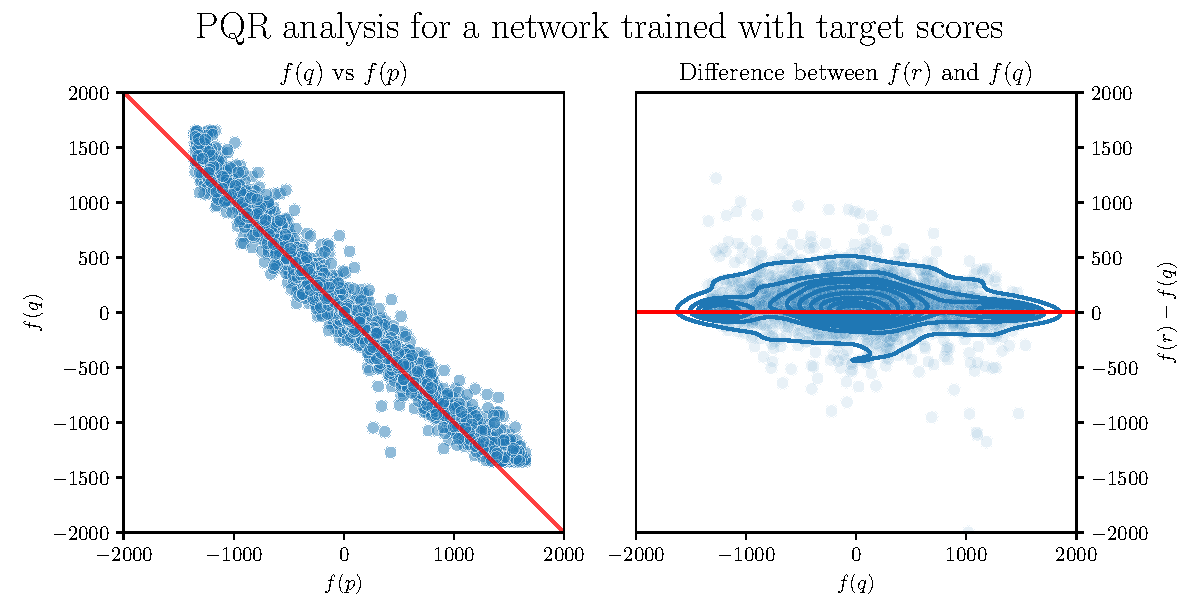
\includegraphics[width=\textwidth]{./dynamic/output/pqr_eval.pdf}}
\caption{Analysis of $N=4000$ PQR samples using a model trained with target scores and the feature set \featureset{All}.}
\label{pqr-eval}
\end{figure}

\newpage
\textbf{Experiment.} I will train the canonical \featureset{All} feature set with this method in two ways:

\begin{enumerate}[label=\bf\Alph*.]
\item \textbf{Train from scratch.} The network is initialized with random weights and trained with the PQR method. This is what the original authors did, and I do not expect to reach the performance of models trained with the evaluations method. Using precomputed evaluations as a target is a lot simpler for the model, since it only has to learn to mimic the scores.

\item \textbf{Continue from a checkpoint.} A strong checkpoint trained with the other method is used to initialize the network. This way, the network does not have to learn too much at once and may enable it to improve the existing parameters. I believe that two scenarios are likely to happen: the model improves very slowly, or it completely forgets what it have learned before and ends up like a model trained from scratch. The best scenario is that the model improves slowly, proving that it can be used to further optimize existing models.
\end{enumerate}

The training data is not filtered the same way as with target scores, where it was known that captures and checks are detrimental. When choosing a random position $R$ from a position $P$, the number of available moves to choose from is $m$ (including $P \rightarrow Q$). Given a parameter $M$, a training sample is skipped if $m < M$. The reasoning behind $M$ is that the bigger the pool to choose from, the more likely it is to find a move that is worse than $P \rightarrow Q$. Note that $M \geq 2$ since otherwise there is only one available move.

Choosing fixed values of $M$ is not ideal, since the number of available moves varies throughout the game. A value of $M$ will be chosen for every turn in the game, based on the distribution of available moves for that particular turn and color. It is known that the white player has more available moves in average than the black player, so $M$ will be different for each.

Four networks will be trained from scratch where $M$ is chosen to filter 0\%, 25\%, 50\% and 75\% of samples with the least available moves for that turn. In figure \ref{avg-moves} we can see the value of $M$ changing throughout the game for each quantile. Note that when $p=0$, $M=2$ in every turn, so no filtering is done. \\

\begin{figure}[H]
\centering
\makebox[\textwidth]{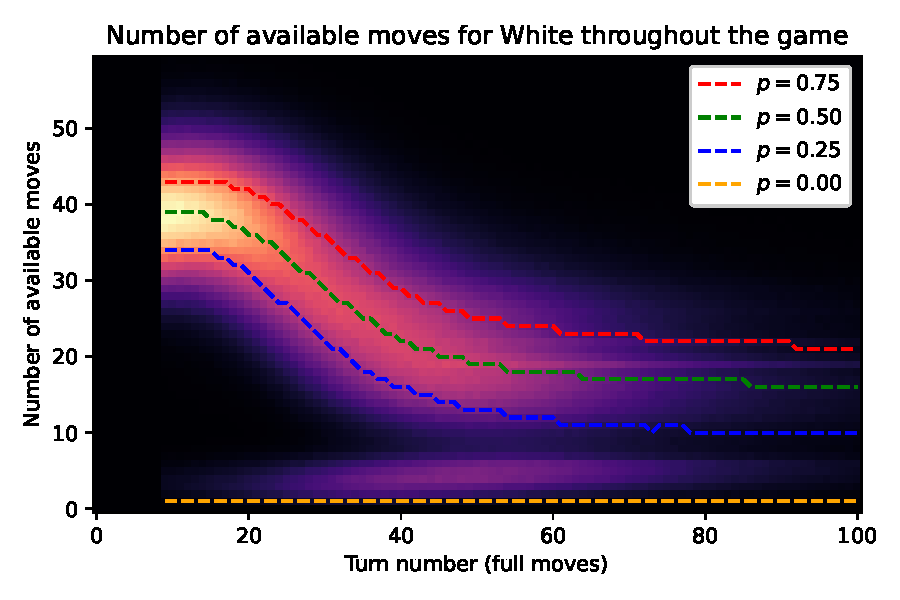
\includegraphics[width=\textwidth]{./dynamic/output/avg_moves.pdf}}
\caption{Heatmap showing the number of available moves for white throughout 100 turns (full moves). The color gradient indicates the density of occurrences in the dataset (N=25M) for positions with a certain number of available moves in a given turn. The plot for black is not shown because it is very similar. The dataset provides positions that start at turn 9.}
\label{avg-moves}
\end{figure}

\newpage
\textbf{(A) Results.} The networks are able to learn with the PQR method from scratch, without the use of existing evaluations like the other method. In figure \ref{pqr-evolution}, we can see the evolution of the ratings of each of the networks trained, along with a network trained with target scores.

\begin{figure}[H]
\centering
\makebox[\textwidth]{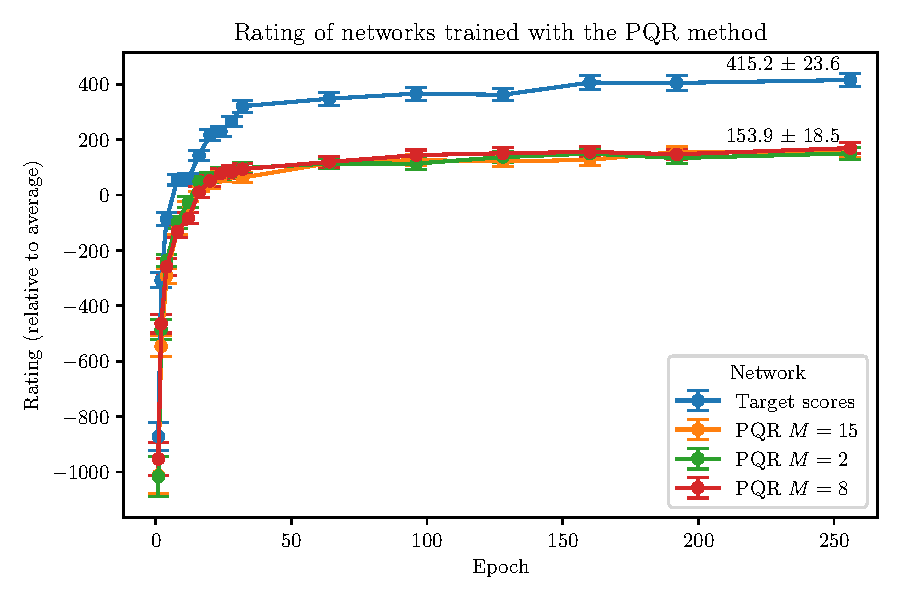
\includegraphics[width=\textwidth]{./dynamic/output/pqr_comparison.pdf}}
\caption{Performance of networks trained from scratch using the PQR method varying the filtering parameter ($p=0,\ 0.25,\ 0.5,\ 0.75$). A network trained with target scores is shown for comparison.}
\label{pqr-evolution}
\end{figure}

The target scores method outperforms the best PQR network by $235 \pm 41$ rating. This result was anticipated, since the target scores method is a lot simpler for the network to learn.

Contrary to what was expected, the larger the pool of moves to choose from (higher values of $p$), the worse the network performs. It was expected that with a higher $M$, it was more likely to find a move that was worse than $P \rightarrow Q$, but this was not the case. A possible explanation is that the positions located in the bottom cloud of the distribution in figure \ref{avg-moves} are good training samples for this method. In the other method, this positions were excluded since most are check positions. The experiment was run again including check positions but the results were the same. \\

\newpage
When looking at the behaviour of $f$ in figure \ref{pqr-scratch}, it does resemble what we expect to happen, a negative correlation between $f(P)$ and $f(Q)$ and a positive difference between $f(R)$ and $f(Q)$. However, the correlation is a lot more spread out, specially in \mbox{$f(P)=-f(Q)$}, which is crucial that they are as close as possible since the network would be predicting different scores for the same position but the other perspective.

A possible improvement could be to try to increase the weight of the \mbox{$f(P)=-f(Q)$} inequalities in the loss function, to force the network to be more like the target scores method. This means reducing the spread in the left plot and give less importance to high differences of \mbox{$f(R)-f(Q)$} since the values should not be as extreme. This is left for future work.

\begin{figure}[H]
\centering
\makebox[\textwidth]{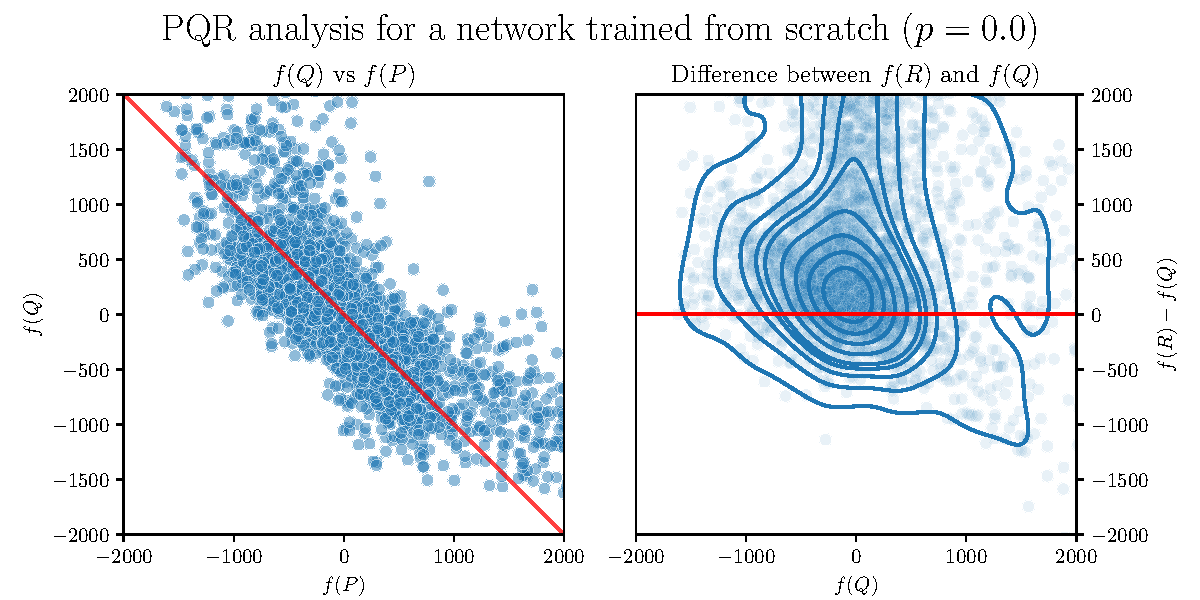
\includegraphics[width=\textwidth]{./dynamic/output/pqr_scratch.pdf}}
\caption{Analysis of $N=4000$ PQR samples using the epoch 256 of the model trained from scratch with no filtering ($p=0.0$) and the feature set \featureset{All}.}
\label{pqr-scratch}
\end{figure}

Of course everything boils down to the dataset, and the dataset used is not ideal for PQR. There are no guarantees that the $P \rightarrow R$ move is not similar in strength or in fact worse than $P \rightarrow Q$. Not only that, but the scale is not the same for all samples. Positions that have a small but significant difference in strength are being penalized the same way as more extreme ones. Trying to filter by the number of available moves did not work, so there is probably no way around it. \\

A good dataset for PQR can be generated using multiple lines of play (maybe dozens), and only include samples where there is a significant difference in strength between the $P \rightarrow Q$ and $P \rightarrow R$ moves. This also can prevent zugzwang\footnote{A zugzwang position occurs when any move a player can make, worsens their position.} positions from being included. It is necessary to decide what threshold is considered significant. One may analyze the distribution of differences and find something good, but in the end we are trying to convey this information to the network, which is what target scores already does, and better. Also, to generate a new dataset with billions of samples a lot of time and compute resources are required. \\

\textbf{(B) Results.} The checkpoint used to continue training is the epoch 256 of the network trained with target scores that appear in figure \ref{pqr-evolution} (rightest purple dot). The training was done for four different values of learning rate: $0.0005$ (previous initializer), $0.0003$, $0.0001$ and $0.00005$. Different values were used to make sure the network does not forget \enquote{too fast} what it has learned before. The results are shown in figure \ref{pqr-ckp}.

\begin{figure}[H]
\centering
\makebox[\textwidth]{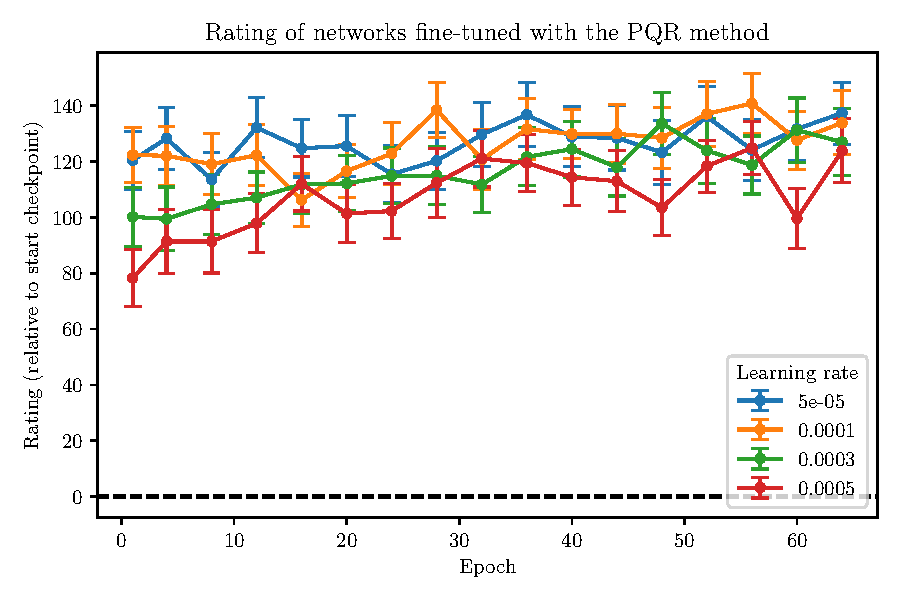
\includegraphics[width=\textwidth]{./dynamic/output/pqr_ckp.pdf}}
\caption{Performance of networks fine-tuned with the PQR method, starting from a target scores checkpoint. The dotted line represents the rating of the checkpoint, which all ratings are relative to.}
\label{pqr-ckp}
\end{figure}

There are a few things to notice in this graph. First, there is a sudden jump from the checkpoint to the first epoch. Since the checkpoint is the starting point, all networks jump in the first epoch to +100 rating. This is suprising, since I expected the network to either improve very slowly or forget what it has learned before.
Second, it shows that there is an upwards trend, which is good. This means that we can use the PQR fine-tune method to further optimize existing models.
Third, the lower the learning rate, the better the network performs. This is expected, since we don't want the network to deviate too fast from the original network. At the same time, it is a bit strange since the steps are not that big to have it gain 100 elo in just one epoch (6103 gradient updates).

I believe that the starting checkpoint was not very strong, and changing to PQR allowed it to get out of a local minimum that it was stuck in. The validation of this hypothesis is left for future work. To explore this further, one could intercalate training between target scores and PQR, to see if it helps the network improve faster.


%\subsection{Active neurons}
%medir si hay feature sets que no usen neuronas, que esto disparo el uso de HalfTopK
%average number of features enabled by feature set (cantidad y porcentaje)
%measure updates per move average and refreshes average per FS
%[ESTO PONERLO EN EL APPENDIX]


%%%%%%%%%%%%%%%%%%%%%%%%%%%%%%%%%%%%%%%%%%%
%%%%%%%%%%%%%%%%%%%%%%%%%%%%%%%%%%%%%%%%%%%
%%%%%%%%%%%%%%%%%%%%%%%%%%%%%%%%%%%%%%%%%%%
%%%%%%%%%%%%%%%%%%%%%%%%%%%%%%%%%%%%%%%%%%%
%%%%%%%%%%%%%%%%%%%%%%%%%%%%%%%%%%%%%%%%%%%
%%%%%%%%%%%%%%%%%%%%%%%%%%%%%%%%%%%%%%%%%%%
%%%%%%%%%%%%%%%%%%%%%%%%%%%%%%%%%%%%%%%%%%%
%%%%%%%%%%%%%%%%%%%%%%%%%%%%%%%%%%%%%%%%%%%
%%%%%%%%%%%%%%%%%%%%%%%%%%%%%%%%%%%%%%%%%%%
%%%%%%%%%%%%%%%%%%%%%%%%%%%%%%%%%%%%%%%%%%%
%%%%%%%%%%%%%%%%%%%%%%%%%%%%%%%%%%%%%%%%%%%


% \noindent\makebox[\linewidth]{\rule{\paperwidth}{0.4pt}}
% 
% Esto de abajo son notas. No se si hacerlo o no... quizas es mucho
% 
% \noindent\makebox[\linewidth]{\rule{\paperwidth}{0.4pt}}
% 
% \subsection{Attacks / Threats}
% 
% as bitsets per piece type
% number of attacks
% 
% \subsection{mas supongo?}
% 
% \subsection{Symmetry? / Relativity?}
% 
% \textbf{Motivation.}
% 
% BUCKETING
% 
% Medir el impacto de agregar simetría al fs. Red mas chica, inf mas rapida, mejor perf?
% 
% probar simetria, eventualmente probar con el mejor feature set de arriba, a ver si mejora poniendo a cada bloque individual simetria
% 
% \featureset{Half-Relative(H|V|HV)King-Piece}?
% 
% inspired by KP, build features relative to the position of the $\king$ King
% 
% \subsection{Statistical features?}
% 
% Define \featureset{k-All-All}
% 
% \featureset{King-All} is a subset of \featureset{All-All}.
% 
% Top P
% 
% Hacer un subset de \featureset{AA} (589824).
% 
% \begin{itemize}
% \item Destilar?
% \item Probar si es lo mismo quedarse con el TOP K de las mas comunes o con las que dice el performance.
% \item Catboost? PCA?
% \end{itemize}
